\documentclass[oneside,12pt]{report}  

% the dimensions of the page
\textheight=9.25in \topmargin=-0.5in   %See note in Chapter 8 of Sample Report about "Page scaling" option in Adobe
\textwidth=6.0in
\oddsidemargin=0.3in
\evensidemargin=0.3in  % Needed to balance even and odd pages in twoside print copy


% Useful packages
\usepackage{dtklogos}
\usepackage{amsmath}
\usepackage{bm}
%\usepackage[colorlinks=true,pagebackref,linkcolor=blue]{hyperref}
\usepackage{amsfonts}
\usepackage{amsthm}
\usepackage{amsmath}
\usepackage{algorithm}
\usepackage{algorithmic}
\usepackage{graphicx}
\usepackage{subfigure}
\usepackage{caption}
\usepackage{excludeonly}

\usepackage{graphicx} 

%\usepackage{doc}
%% Following sets up logic and formatting for conditional twoside copying
%\usepackage{ifthen, color, fancyvrb}
%\usepackage{nextpage}\pagestyle{plain}
%\newcommand\myclearpage{\cleartooddpage
%  [\thispagestyle{empty}]
%  }

\DeclareMathOperator*{\argmin}{arg\ min}
\DeclareMathOperator*{\sign}{sign}

% Note special alternative codes for using TWO bibliographies; see cautionary note in
\DeclareGraphicsExtensions{ps,eps,PNG,png}

% Theorem-like command definitions:
\newtheorem{theorem}{Theorem}[chapter]
\newtheorem{lemma}{Lemma}[chapter]
\newtheorem{definition}{Definition}  % Note, this italicizes everything

% Print the chapter and sections in the toc
\setcounter{tocdepth}{1}

% Specify which files to typeset for this run (note that overall pagination is preserved)
%\includeonly{chapter1, chapter2}
% Specify which files NOT to typeset for this run (note that overall pagination is preserved)
%\excludeonly{}

% Groundwork for allowing double-sided copying with blank versos
\def\prefacesection#1{
\chapter*{#1}
\addcontentsline{toc}{chapter}{#1}
}

\begin{document}


\def\thefootnote{\fnsymbol{footnote}}

\thispagestyle{empty}

% The numbers below controls the amount of space between the following sections
\def\shiftdowna{0.32in}  % Adjust for balance
\def\shiftdownb{0.22in}  % Adjust for balance

% Set up the boiler plate at the top of the page

\begin{center}
\textbf{{\large Mathematical Modeling and Consulting }}\\

\vspace \shiftdowna

\includegraphics[width=0.5\textwidth]{jhu.png}\\

% Home Department
\vspace \shiftdowna
\underline {Sponsor}\\ 
\vspace{5pt}
\textbf{\large Jabre Capital} \\
\vspace\shiftdowna
\textbf{{Progress Report}}

% TITLE
\vspace \shiftdowna
\textbf{{\Large Portfolio Optimization based on PCA analysis}}

% STUDENTS
\vspace{0.35in}
\underline {Team Members}\\
\vspace{5pt}
Tianyu Luo (Project Manager),Engineering Management Department\\
\texttt{tluo3@jhu.edu} \\
\vspace{10pt}
Zichan Wang(Report Coordinator), Engineering Management Department\\
\texttt{zichan.wang@gmail.com}\\
\vspace{10pt}
Yixuan Da(Report Coordinator), Financial Mathematics Department\\
\texttt{dayixuan2010@gmail.com}\\

% INSTRUCTOR
\vspace \shiftdownb
\underline {Academic Mentor} \\
\vspace{5pt}
\text{Dr.~N.~H.~Lee}, Applied Mathematics and Statistics\\
\texttt{nhlee@jhu.edu}

% Consultants
%\vspace \shiftdownb 
%\underline {Consultant}\\
%\vspace{5pt}
%Jason Bourne\\

% DATE
\vspace \shiftdowna
Date: Last Complied on \today

\end{center}

\vfill  %Fill page to force following note to bottom
\footnoterule
\noindent \small{This project was supported by Jabre Capital.}

% Begin ABSTRACT
\ifthenelse{\boolean{@twoside}}{\myclearpage}{}
\prefacesection{Abstract}
The stock market is a financial game of winners and losers. Using the multivariate statistical methods of principal component analysis (PCA), we aim to find out the problems of Jabre Capital Partners’ stock investment portfolio and choice. Since the unsystematic risk is a risk that can be avoided and the market does not compensate for taking such risks, our work focuses on the evaluation of the unsystematic risk of Jabre Capital Partners. 

We divided our work into two stages: first is to analyze the diversification and unsystematic risk of the 21 stocks that company held for entire year, second is to analyze the stock portfolio changes from quarter to quarter in order to observe the diversification improved or not. Since PCA can find structure in the covariance or correlation matrix and uses this structure to locate low-dimensional subspaces containing most of the variation in the data, we can tell whether the stock portfolio is diversified or not, that is whether the unsystematic risk is low or not.

% Begin ACKNOWLEDGMENTS
\ifthenelse{\boolean{@twoside}}{\myclearpage}{}
\prefacesection{Acknowledgments}
We would like to extend many thanks to all those at Mathematical Modelling and Consulting class who helped and supported us through the project, and have made it an enjoyable and rewarding experience.

Firstly, we would like to extend our deepest gratitude to our supervisor ~N.~H.~Lee for his continuous encouragement, general support and mentoring throughout the project. He has taught us how to solve problems quickly, express ideas clearly, and communicate with people efficiently.

Second, we would also like to thank Yahoo Finance, its support and valuable hints gave us useful information and helped us spark new ideas. 

Thank you very much to all of you for having made this experience interesting, rewarding and enjoyable.


% Table of contents, List of Figures, and List of Tables.
\ifthenelse{\boolean{@twoside}}{\myclearpage}{}
\tableofcontents

\ifthenelse{\boolean{@twoside}}{\myclearpage}{}
\listoffigures

\ifthenelse{\boolean{@twoside}}{\myclearpage}{}
\listoftables


\renewcommand{\thefootnote}{\arabic{footnote}}
\setcounter{footnote}{0}

\ifthenelse{\boolean{@twoside}}{\myclearpage}{}
\include{A_Introduction}
\chapter{Introduction}\label{Introduction}
Jabre Capital Partners is an alternative asset management platform founded in 2006. The Group offers a diversified range of investment management services and products, including Cayman-based collective investment schemes, UCITS IV regulated strategies, and individually managed accounts, to a broad network of institutional and high net worth clients. In addition, the Group provides discretionary investment management and advisory services to private clients.

As of December 31th 2010, Jabre Capital had portfolio value of \$4,133,365,000. A year later, the portfolio value was only \$793,966,000.In one year, the hedge fund's value was down by around 80\%, which made it among the 10 worst hedge funds 2011.   
\include{B_TechnicalBackground}
\chapter{Technical Background}\label{Technical Background}
The stock market is a financial game of winners and losers. Is there a method to predict the stock market? Using the multivariate statistical methods of principal component analysis (PCA), we aim to find out the problem of Jabre Capital Partners’ stock investment portfolio and choice. 

Diversifiable risk (also known as unsystematic risk) represents the portion of an asset’s risk that is associated with random causes that can be eliminated through diversification. While the non-diversifiable risk (also known as systematic risk) is the relevant portion of an asset’s risk attributable to market factors that affect all firms such as war, inflation, international incidents, and political events. In the other word systematic risk is beyond the control of investors and cannot be mitigated to a large extent. In contrast to this, the unsystematic risk can be mitigated through portfolio diversification. Since the unsystematic risk is a risk that can be avoided and the market does not compensate for taking such risks, our work focuses on the evaluation of the unsystematic risk of Jabre Capital Partners.

Principal component analysis (PCA) is a mathematical procedure that uses an orthogonal transformation to convert a set of observations of possibly correlated variables into a set of values of linearly uncorrelated variables called principal components. Using PCA, we will combine related factor, which is weekly return performance of the stocks, into a smaller number of key components largely responsible for the variations observed. Since PCA can find structure in the covariance or correlation matrix and uses this structure to locate low-dimensional subspaces containing most of the variation in the data, we can tell whether the stock portfolio is diversified or not, that is whether the unsystematic risk is low or not. 

\include{C_ProblemStatement}
\chapter{Problem Statement}\label{Problem Statement}
According to a talk with the company fund manager, Philippe Jabre, it was known that the company implemented a conservative investment strategy in year 2011 in order to reduce unsystematic risk by improving the portfolio diversification. This strategy has been confirmed by Figure 1 which implies that the fund manager had changed the stock portfolio from quarter to quarter. However, this change did not prevent the portfolio value and investment return from skyfalling. In addition, due to the low portfolio value and the low return of investment, the company was limited to invest in a large numbers of stocks to increase diversification which deteriorated the situation even more. 

\begin{figure}[h]
    \begin{center}
        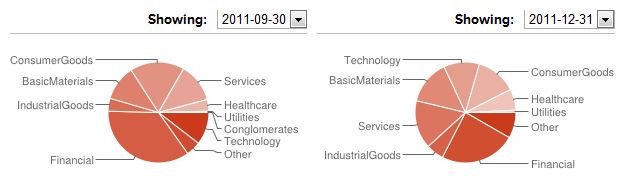
\includegraphics[width=\textwidth]{2.png}
    \end{center}
    \caption{Jabre Capital's Portfolio Selection in 2011}
    \label{fig:piechart}
\end{figure}

First, Mr. Jabre did not truly grab the essence of the diversification of the stock. Diversification is aimed to decrease the unsystematic risk of a portfolio by introducing diversified stocks. However, investing in a large number of different stocks cannot guarantee the diversification of the portfolio. In addition, if the stocks performances are positively related to each other, the portfolio risk can be increased rather than decreased.

Second, apart from the stock number and diversification from a general aspect, the company has problem in stock selection in different industries as well. For example, the stocks in bank industry tend to be positively correlated to each other since they usually depend on the monetary policy. As a result, we can decrease the stock number held in bank industry since they have limited diversification and a specific stock can explain a certain pattern of stock performance. However, it is different in IT industry since the stocks’ performances have less correlation to each other. Based on this reason, we need to maximize the diversification of the stock holdings in this industry. As a result, the selection of the stocks in different industries has great impact on the investment performance. 

\include{D_Analysis}
\chapter{Analysis}\label{Analysis}
In order to analyze these problems, we categorize the risk into systematic risk and unsystematic risk. The systematic risk does not depend on individual companies and industry. Thus, it is independent (exogenous). The unsystematic risk depends on the financial position of the individual company, the industry the company is in, and so on. Thus, it is dependent (endogenous). 

After we went through the stock holdings of the company from Yahoo Finance, it has been known that the company invested 418 stocks throughout year 2011 in total. Since this is a huge database, we then divided our work into two stages: first is to analyze the diversification and unsystematic risk of the 21 stocks that company held for entire year, second is to analyze the stock portfolio changes from quarter to quarter in order to observe the diversification improved or not. 

\include{E_Results}
\chapter{Results}\label{Results}
\begin{figure}[ht]
\centering
\subfigure[Eigenvalue of the correlation matrix]{
	%\rule{4cm}{3cm}
        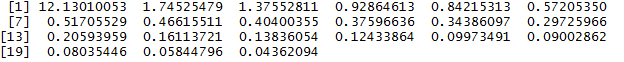
\includegraphics[width=\textwidth]{3.png}
	\label{fig:subfig1}
}
\subfigure[Eigenvector of the correlation matrix(some columns are excluded due to limited space)]{
	%\rule{4cm}{3cm}
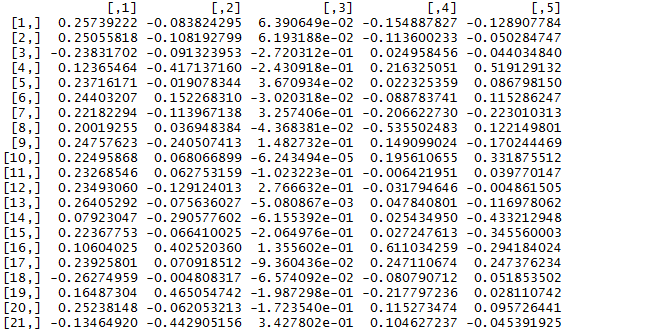
\includegraphics[width=\textwidth]{4.png}
	\label{fig:subfig2}
}
%\subfigure[Plot of Principal Components]{
%	%\rule{4cm}{3cm}
%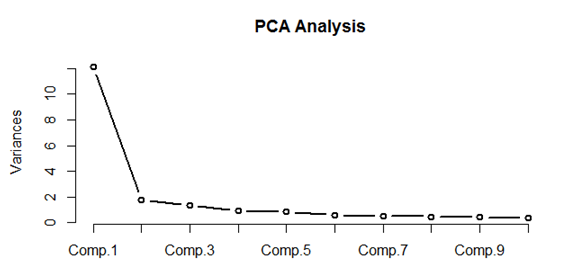
\includegraphics[width=\textwidth]{5.png}
%	\label{fig:subfig3}
%}
\caption[Optional caption for list of figures]{Engenvalue and eigenvector of the correlation matrix}
\label{fig:subfigureExample}
\end{figure}
We conducted the PCA analysis in the following steps:
\begin{enumerate}
\item We standardized the return matrix using R and got the standardized return matrix(51*21),
\item we calculated the correlation matrix,
\item we linearized the correlation matrix into independent eigenvectors and corresponding eigenvalues as shown above, and the plot accordingly.
\end{enumerate}

Because the space is limited, we don't provide the complete eigenvector matrix here. We don't provide the standardized matrix and correlation matrix, either. This information will be provided upon request.
\begin{figure}[ht]
    \begin{center}
        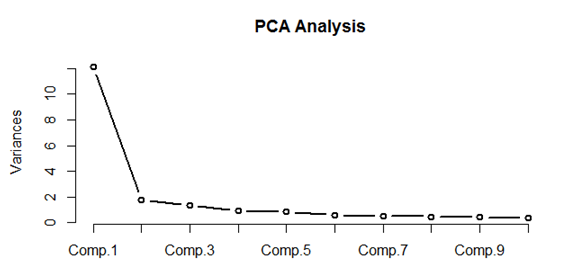
\includegraphics[width=\textwidth]{5.png}
    \end{center}
    \caption{Jabre Capital's Portfolio Selection in 2011}
    \label{fig:eigenvector}
\end{figure}

\include{F_Conclusion}
\chapter{Conclusion}\label{Conclusion}
The PCA analysis result shows that the first three eigenvectors can explain appoxiamately 72.62\% of the variance of the portforlio. So we believe that the correlation among the 21 stocks is relatively high and the portforlio is not well diversified. In this case, the portfolio is more risky than the other well diversified portfolios. 

In the future reseach, we will mainly look into if adding more stocks from different industries, asset classes and commodities will improve the result.

%\include{chapter1}
%\include{chapter2}
%\include{chapter3}
%\include{chapter4}
%\include{chapter5}
%\include{chapter6}


\appendix
\ifthenelse{\boolean{@twoside}}{\myclearpage}{}

\chapter{Lemmas}\label{Lemma}

\chapter{Glossary}\label{Glossary}

\vspace{12pt} 

\vspace{8pt}
\noindent {\bf Principal Component Analysis}.  A mathematical procedure that uses an orthogonal transformation to convert a set of observations of possibly correlated variables into a set of values of linearly uncorrelated variables called principal components. 

\vspace{8pt}
\noindent {\bf Systematic Risk}. The portion of an asset’s risk that is associated with random causes that can be eliminated through diversification. 

\vspace{8pt}
\noindent {\bf Unsystematic Risk}. The portion of an asset’s risk attributable to market factors that affect all firms such as war, inflation, international incidents, and political events. 

%\vspace{8pt} \noindent {\bf Footprint}. The intersection of a visibility cone with the surface of the earth.
%
%\vspace{8pt} \noindent {\bf Great circle of arc}. The shortest path between two points on the surface of the earth. 
%
%\vspace{8pt} \noindent {\bf Groundtrack}.The location of the center of a visibility cone footprint on the surface of the earth.
%
%\vspace{8pt}
%\noindent {\bf Inclination}.  The angle between the normal to the orbit plane
%and the normal to the equatorial plane.
%
%\vspace{8pt} \noindent {\bf LEO}. An orbit with an altitude approximately below 2,000 km.
%
%\vspace{8pt} \noindent {\bf Molniya orbit}. A highly elliptical orbit with an orbital period of half a day.
%
%\vspace{8pt} \noindent {\bf Projection distance}. The distance between the center of the visibility cone footprint and a point of interest projected onto the plane orthogonal to the vector defining the visibility cone center and tangent to the earth surface.
%
%\vspace{8pt}
%\noindent {\bf Right ascension of the ascending node}. The angle
%between the unit vector $\bm{X}$ and the point where the satellite crosses the
%ascending node, measured counterclockwise when viewed from the north side of
%the equatorial plane.


\ifthenelse{\boolean{@twoside}}{\myclearpage}{}
\chapter{Abbreviations}\label{Abbreviations}


\noindent PCA.  Principal Component Analysis

\vspace{5pt}

%\noindent ECR.  Earth-centered rotating frame
%
%\vspace{5pt}
%
%\noindent LEO.  Low Earth Orbit  
%
%\vspace{5pt}
%
%\noindent RAAN. Right ascension of the ascending node
%
%\vspace{5pt}

%\endinput

% Add your bibliography to Contents
\ifthenelse{\boolean{@twoside}}{\myclearpage}{\newpage}
\addtocontents {toc}{\protect \contentsline {chapter}{REFERENCES}{}}
\addcontentsline{toc}{chapter}{Selected Bibliography Including Cited Works}  

% Bibliography must come last.
\bibliographystyle{plain}
\renewcommand\bibname{Selected Bibliography Including Cited Works}
\nocite{*}  % List ALL references in your references, not just the ones cited in the text.
% This scheme automatically alphabetizes the Bibliography.
\bibliography{Biblio}
\end{document}
